\documentclass[11pt,a4paper]{article}
\usepackage[a4paper,margin=22mm]{geometry}
\usepackage{fontspec}
\usepackage{xeCJK}
\usepackage{amsmath,amssymb,amsfonts,mathtools,bm}
\usepackage{booktabs,array,longtable,multirow,tabularx}
\usepackage[dvipsnames]{xcolor}
\usepackage{graphicx}
\usepackage{tikz}
\usetikzlibrary{arrows.meta,positioning,fit,backgrounds,calc,shapes.geometric}
\usepackage{enumitem}
\usepackage{hyperref}
\usepackage{fancyhdr}
\usepackage{titlesec}
\usepackage{tcolorbox}
\usepackage{lastpage}
% \usepackage{newtxtext} % removed: conflicts with fontspec in XeLaTeX
\usepackage{mathrsfs}

\setmainfont{TeX Gyre Termes}
\setsansfont{TeX Gyre Heros}
\setmonofont{DejaVu Sans Mono}
\setCJKmainfont{Noto Serif CJK KR}
\setCJKsansfont{Noto Sans CJK KR}

\definecolor{TitleBlue}{HTML}{143D6B}
\definecolor{AccentTeal}{HTML}{0F7C82}
\definecolor{SoftBlue}{HTML}{EAF3FB}
\definecolor{SoftTeal}{HTML}{EAF8F6}
\definecolor{SoftGray}{HTML}{F3F5F7}
\definecolor{LineGray}{HTML}{D5DADF}
\definecolor{WarnOrange}{HTML}{C97A00}
\definecolor{DeepRed}{HTML}{8F2D2D}

\hypersetup{colorlinks=true,linkcolor=TitleBlue,urlcolor=AccentTeal,citecolor=TitleBlue,pdftitle={CMP Profile Control H-infinity Design Specification},pdfauthor={OpenAI}}
\pagestyle{fancy}
\fancyhf{}
\lhead{\textcolor{TitleBlue}{CMP Profile Control $H_{\infty}$ Design Specification}}
\rhead{\textcolor{AccentTeal}{XeLaTeX EN Edition}}
\cfoot{\textcolor{gray}{\thepage/\pageref{LastPage}}}
\setlength{\headheight}{14pt}

\titleformat{\section}{\Large\bfseries\color{TitleBlue}}{\thesection.}{0.6em}{}
\titleformat{\subsection}{\large\bfseries\color{AccentTeal}}{\thesubsection}{0.6em}{}
\titleformat{\subsubsection}{\normalsize\bfseries\color{TitleBlue}}{\thesubsubsection}{0.6em}{}
\titlespacing*{\section}{0pt}{1.2em}{0.6em}
\titlespacing*{\subsection}{0pt}{0.9em}{0.4em}

\renewcommand{\arraystretch}{1.28}
\setlength{\parindent}{0pt}
\setlength{\parskip}{5pt}

\newcommand{\R}{\mathbb{R}}
\newcommand{\norm}[1]{\left\lVert #1 \right\rVert}
\newcommand{\diag}{\operatorname{diag}}
\newcommand{\e}{\mathrm{e}}

\begin{document}

\begin{titlepage}
\pagecolor{white}
\begin{tikzpicture}[remember picture,overlay]
\fill[SoftBlue] (current page.north west) rectangle ([yshift=-6.5cm]current page.north east);
\fill[AccentTeal] ([yshift=-6.5cm]current page.north west) rectangle ([yshift=-7.0cm]current page.north east);
\draw[TitleBlue,line width=1.2pt] ([xshift=1.2cm,yshift=-1.2cm]current page.north west) rectangle ([xshift=-1.2cm,yshift=1.2cm]current page.south east);
\end{tikzpicture}

\vspace*{2.0cm}
{\fontsize{24}{30}\selectfont\bfseries\color{TitleBlue} CMP Profile Control $H_{\infty}$\par}
\vspace{0.2cm}
{\fontsize{22}{28}\selectfont\bfseries\color{TitleBlue} Design Specification\par}
\vspace{0.5cm}
{\fontsize{15}{20}\selectfont\color{AccentTeal} Integrated R2R + InRun Review Edition (v4.2)\par}

\vspace{1.0cm}
\begin{tcolorbox}[colback=white,colframe=TitleBlue,boxrule=0.8pt,arc=2mm]
\small
This XeLaTeX edition was rebuilt specifically to avoid equation corruption and formula-in-figure decoding failures. All equations, figure labels, and block-diagram annotations are rendered directly by LaTeX rather than embedded as pre-rasterized text. The technical direction follows the uploaded integrated review edition: InRun control is the primary real-time loop, while R2R acts as the supervisory adaptation layer.
\end{tcolorbox}

\vspace{0.8cm}
\begin{tabularx}{\textwidth}{>{\bfseries}p{3.3cm}X}
Document type & Technical design specification for hierarchical CMP profile control \\
Scope & 11 pressure inputs including retaining ring, 21 profile outputs, turn-wise and wafer-wise control \\
Primary design frame & Discrete-time robust control with hard actuator constraints and real-time disturbance rejection \\
Deliverables & English PDF, Korean PDF, and XeLaTeX source \\
Date & 2026-03-21 \\
\end{tabularx}

\vfill
{\large\bfseries\color{TitleBlue} Key message}\par
\vspace{0.2cm}
{\large InRun target tracking must close the fast loop inside the wafer; R2R should provide baseline adaptation, wear compensation, and supervisory recipe correction.}\par

\vspace{1.0cm}
{\color{gray}Prepared as a formula-safe XeLaTeX master source.}
\end{titlepage}

\tableofcontents
\newpage

\section{Document Status and What Was Corrected}
The uploaded integrated review edition states that the document scope was expanded from a purely wafer-to-wafer formulation to a hierarchical architecture in which InRun profile control is the primary real-time objective and R2R is the supervisory layer. It also states that the revision corrected LaTeX breakage, notation inconsistencies, and delay-notation ambiguity.\footnote{See the uploaded integrated review edition for the scope statement, deliverables, and table of contents.} The present XeLaTeX build preserves that direction while making all equations native LaTeX objects so that the rendered PDF no longer contains broken math text in figures or body formulas.\par

\subsection{Revision history}
\rowcolors{2}{SoftGray}{white}
\begin{longtable}{p{1.5cm}p{1.8cm}p{8.4cm}p{3.0cm}}
\toprule
\textbf{Version} & \textbf{Date} & \textbf{Summary of changes} & \textbf{Review source} \\
\midrule
\endhead
v1 & 2026-03-21 & Initial $H_{\infty}$ CMP profile-control specification in Markdown/LaTeX style. & Initial draft \\
v2 & 2026-03-21 & Added explicit R2R scope, metrology delay, structured wear uncertainty, non-square MIMO sensitivity, hard pressure and slew constraints, anti-windup, observer structure, generalized-plant partitioning, and SVD/null-space analysis. & Review set 1--2 \\
v3 & 2026-03-21 & Added implementation guidance for delay-state growth, reduced-space design with original-space hard constraints, and delayed-measurement observer roll-forward handling. & Implementation review \\
v4 & 2026-03-21 & Added review-to-revision traceability. & Traceability request \\
v4.1 & 2026-03-21 & Corrected formula breakage, index notation, title mismatch, and baseline formulation consistency; repackaged as polished XeLaTeX editions in English and Korean. & Full document review \\
v4.2 & 2026-03-21 & Integrated InRun-primary framing, verification plan, and deployable-baseline guidance into a single master source. & Integrated review edition \\
\bottomrule
\end{longtable}

\subsection{Review-to-revision traceability}
\begin{itemize}[leftmargin=1.5em]
\item Time-scale ambiguity $\rightarrow$ resolved by separating wafer index $k$ from in-wafer turn index $j$ and by defining a hierarchical control architecture.
\item Metrology delay omission $\rightarrow$ resolved by explicit delayed-measurement equations and delay-state augmentation.
\item Non-square sensitivity misuse $\rightarrow$ replaced with output-side and input-side sensitivity definitions.
\item Pressure non-negativity and slew constraints $\rightarrow$ enforced as hard actuator constraints, not soft preferences.
\item Anti-windup omission $\rightarrow$ addressed with back-calculation and conditional-integration guidance.
\item Weak wear modeling $\rightarrow$ refined into slowly varying structured uncertainty.
\item Missing controllability interpretation $\rightarrow$ supplemented with SVD-based mode selection and residual monitoring.
\item Generalized-plant incompleteness $\rightarrow$ repaired by explicit partitioned state-space equations.\end{itemize}

\section{Scope and Control Time Scale}
\subsection{Primary scope}
This specification targets hierarchical CMP profile control with two coupled time scales:
\begin{enumerate}[leftmargin=1.6em]
\item \textbf{InRun (in-wafer) control}: the primary control layer that updates pressure during polishing of the same wafer at turn, sector, or short control-interval rate.
\item \textbf{Run-to-run (R2R) control}: the supervisory layer that updates the baseline recipe from wafer to wafer.
\end{enumerate}
The more important production objective is the InRun profile-tracking problem: define a target profile or target profile trajectory, measure the within-wafer deviation from that target, and compute bounded pressure corrections fast enough to suppress the error before the wafer completes polishing.

\subsection{Role split between InRun and R2R}
R2R supplies a good baseline recipe and adapts slowly to incoming-wafer changes, wear drift, and lot-to-lot shifts. InRun rejects fast disturbances, compensates within-wafer nonuniformity, and drives the measured profile toward the desired target during the same wafer. This is the central design stance of the integrated review edition.\par

\begin{figure}[h!]
\centering
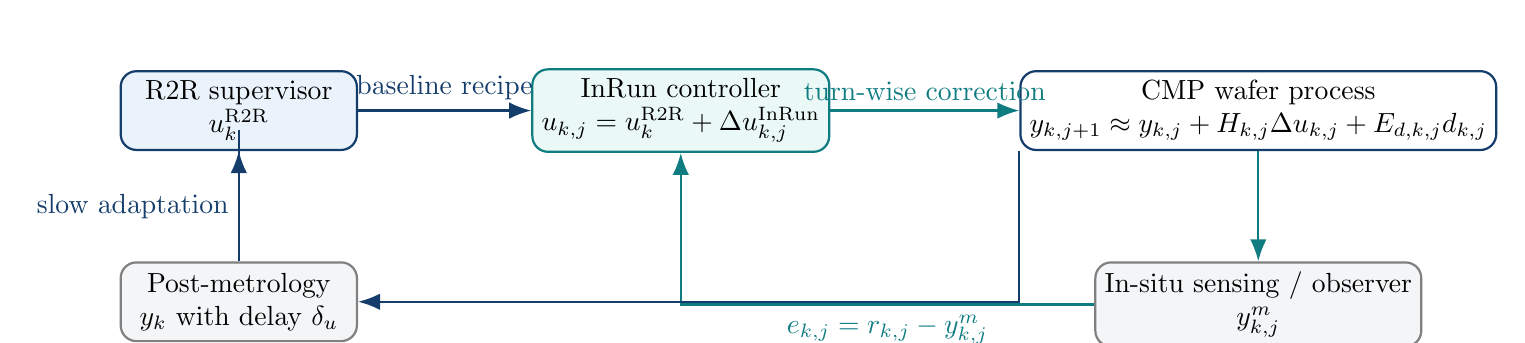
\begin{tikzpicture}[
node distance=8mm and 10mm,
box/.style={draw,rounded corners=2mm,thick,align=center,minimum height=10mm,minimum width=30mm},
arr/.style={-{Latex[length=2.8mm]},thick}
]
\node[box,fill=SoftBlue,draw=TitleBlue] (recipe) {R2R supervisor\\$u_k^{\mathrm{R2R}}$};
\node[box,fill=SoftTeal,draw=AccentTeal,right=22mm of recipe] (sum) {InRun controller\\$u_{k,j}=u_k^{\mathrm{R2R}}+\Delta u_{k,j}^{\mathrm{InRun}}$};
\node[box,fill=white,draw=TitleBlue,right=24mm of sum] (plant) {CMP wafer process\\$y_{k,j+1}\approx y_{k,j}+H_{k,j}\Delta u_{k,j}+E_{d,k,j}d_{k,j}$};
\node[box,fill=SoftGray,draw=gray,below=14mm of plant] (sensor) {In-situ sensing / observer\\$y^m_{k,j}$};
\node[box,fill=SoftGray,draw=gray,below=14mm of recipe] (metro) {Post-metrology\\$y_k$ with delay $\delta_u$};
\draw[arr,TitleBlue] (recipe) -- node[above,] {baseline recipe} (sum);
\draw[arr,AccentTeal] (sum) -- node[above,] {turn-wise correction} (plant);
\draw[arr,AccentTeal] (plant) -- (sensor);
\draw[arr,AccentTeal] (sensor.west) -| node[pos=0.25,below,] {$e_{k,j}=r_{k,j}-y^m_{k,j}$} (sum.south);
\draw[arr,TitleBlue] (plant.south west) |- (metro.east);
\draw[arr,TitleBlue] (metro.north) |- node[pos=0.25,left,] {slow adaptation} (recipe.south);
\end{tikzpicture}
\caption{Hierarchical architecture: InRun closes the fast loop inside a wafer, while R2R performs supervisory adaptation across wafers.}
\end{figure}

\subsection{Index meaning}
\[
k\in\{0,1,2,\dots\}
\]
denotes the wafer or run index, while
\[
j\in\{0,1,2,\dots,N_k\}
\]
denotes the in-wafer turn or short control-interval index for wafer $k$.

\section{Plant Definition}
\subsection{Input vector}
The manipulated variable is the pressure command vector
\[
u_k\in\R^{11},\qquad u_k=[u_{1,k},u_{2,k},\dots,u_{10,k},u_{\mathrm{RR},k}]^\top,
\]
where the first ten entries correspond to carrier-head pressure zones and the last entry corresponds to the retaining-ring pressure.

\subsection{Output vector}
The controlled output is the radial profile vector
\[
y_k\in\R^{21},
\]
representing 21 radial sample points or 21 profile-basis coordinates after metrology.

\subsection{Reference and tracking error}
The reference profile is
\[
r_k\in\R^{21},
\]
and the tracking error is
\[
e_k=r_k-y_k.
\]

\section{InRun (In-Wafer) Control Problem Formulation}
\subsection{Turn-wise target profile}
For wafer $k$, let the desired in-wafer target profile at turn $j$ be
\[
r_{k,j}\in\R^{21}.
\]
This target may be a constant final profile applied at every turn, or a scheduled profile trajectory that reflects expected removal progress.

\subsection{Measured profile and error}
Let the available in-situ or observer-reconstructed profile measurement be
\[
y^m_{k,j}\in\R^{21},
\]
and define the InRun tracking error by
\[
e_{k,j}=r_{k,j}-y^m_{k,j}.
\]
If direct 21-point in-situ profile sensing is unavailable, $y^m_{k,j}$ should be interpreted as the estimated profile state reconstructed from motor signals, friction proxies, optical channels, or other side measurements.

\subsection{Incremental control move}
The InRun manipulated variable is the turn-wise pressure correction
\[
u_{k,j}\in\R^{11},\qquad \Delta u_{k,j}=u_{k,j}-u_{k,j-1}.
\]
A practical hierarchical decomposition is
\[
u_{k,j}=u_k^{\mathrm{R2R}}+\Delta u_{k,j}^{\mathrm{InRun}},
\]
where $u_k^{\mathrm{R2R}}$ is the wafer-level baseline recipe and $\Delta u_{k,j}^{\mathrm{InRun}}$ is the real-time within-wafer correction.

\subsection{Local InRun model}
A generic in-run model may be written as
\begin{align*}
x^{\mathrm{in}}_{k,j+1} &= A^{\mathrm{in}}_{k,j}x^{\mathrm{in}}_{k,j}+B^{\mathrm{in}}_{k,j}\Delta u_{k,j}+B^{\mathrm{in}}_{d,k,j}d_{k,j},\\
y^m_{k,j} &= C^{\mathrm{in}}_{k,j}x^{\mathrm{in}}_{k,j}+v_{k,j},
\end{align*}
where $d_{k,j}$ represents real-time process disturbances and $v_{k,j}$ is measurement noise. For engineering interpretation, an equivalent profile-increment form is
\[
y_{k,j+1}\approx y_{k,j}+H_{k,j}\Delta u_{k,j}+E_{d,k,j}d_{k,j}.
\]

\subsection{Real-time disturbance classes}
The disturbance term $d_{k,j}$ should include local incoming-film nonuniformity revealed during polishing, slurry-flow variation, pad hydrodynamic fluctuation, retaining-ring edge-contact transients, friction drift, thermal drift, and sensor bias drift. Consequently, the controller must be designed for both reference tracking and real-time disturbance rejection.

\subsection{InRun control objective}
A suitable finite-horizon objective over a wafer is
\begin{align*}
\min_{\{u_{k,j}\}}\;\sum_{j=0}^{N_k} \Big(&\norm{W_{e,j}(r_{k,j}-y_{k,j})}_2^2+\norm{W_{\Delta u,j}(u_{k,j}-u_{k,j-1})}_2^2\\
&+\norm{W_{u,j}(u_{k,j}-u_k^{\mathrm{R2R}})}_2^2\Big),
\end{align*}
subject to
\[
u_{\min}\le u_{k,j}\le u_{\max},\qquad \Delta u_{\min}\le u_{k,j}-u_{k,j-1}\le \Delta u_{\max}.
\]
This objective expresses four simultaneous requirements: target tracking, smooth pressure motion, limited departure from the supervisory recipe, and strict actuator feasibility at all times.

\subsection{Why InRun dominates performance}
If the controller waits until the next wafer to correct an error that was already visible during the current wafer, the error has already been printed into the finished profile. Therefore, whenever useful in-situ information is available, R2R alone is insufficient for high-performance profile control.

\section{R2R Model with Metrology Delay}
\subsection{Static baseline model}
The baseline influence-matrix model is
\[
y_k=G_k u_k+d_k,
\]
where $G_k\in\R^{21\times 11}$ is the effective run-dependent influence matrix and $d_k\in\R^{21}$ is the lumped disturbance vector.

\subsection{Delayed metrology model}
In production CMP, the measured profile often becomes available only after a delay of $\delta_u$ runs. A clean statement of the delayed relation is
\[
y_{k+\delta_u}=G_k u_k+d_{k+\delta_u}.
\]
After index shifting,
\[
y_k=G_{k-\delta_u}u_{k-\delta_u}+d_k.
\]
This is the form used when the available measurement at control step $k$ is discussed.

\subsection{Delay-state augmentation}
Define a delay-augmented pressure-history state
\[
x_k^{(d)}=\begin{bmatrix}u_{k-1}\\u_{k-2}\\\vdots\\u_{k-\delta_u}\end{bmatrix},
\]
and include it explicitly in the state-space realization so that the metrology delay is not hidden inside an unstructured disturbance term.

\begin{figure}[h!]
\centering
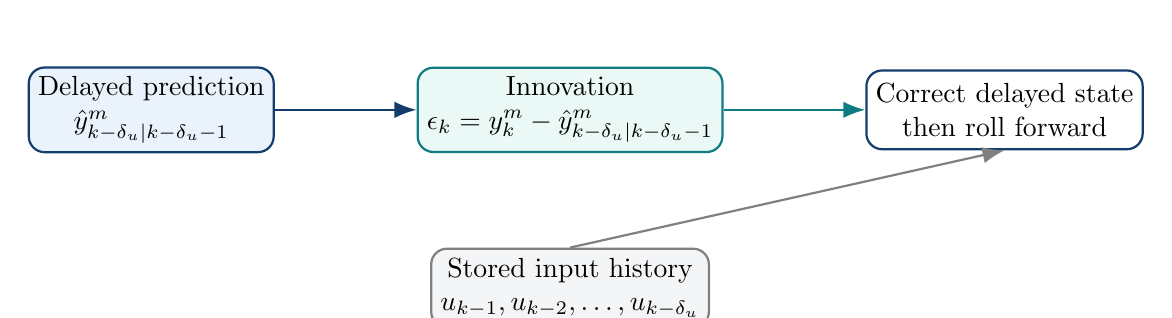
\begin{tikzpicture}[
node distance=8mm and 10mm,
box/.style={draw,rounded corners=2mm,thick,align=center,minimum height=10mm,minimum width=30mm},
arr/.style={-{Latex[length=2.8mm]},thick}
]
\node[box,fill=SoftBlue,draw=TitleBlue] (pred) {Delayed prediction\\$\hat y^{m}_{k-\delta_u\mid k-\delta_u-1}$};
\node[box,fill=SoftTeal,draw=AccentTeal,right=18mm of pred] (innov) {Innovation\\$\epsilon_k=y_k^m-\hat y^{m}_{k-\delta_u\mid k-\delta_u-1}$};
\node[box,fill=white,draw=TitleBlue,right=18mm of innov] (corr) {Correct delayed state\\then roll forward};
\node[box,fill=SoftGray,draw=gray,below=12mm of innov] (hist) {Stored input history\\$u_{k-1},u_{k-2},\dots,u_{k-\delta_u}$};
\draw[arr,TitleBlue] (pred) -- (innov);
\draw[arr,AccentTeal] (innov) -- (corr);
\draw[arr,gray] (hist.north) -- (corr.south);
\end{tikzpicture}
\caption{Delayed-metrology observer logic. The innovation is aligned with the matching delayed prediction and then propagated to the current control step with stored input history.}
\end{figure}

\subsection{Practical baseline assumption}
For first implementation, a one-run effective delay is acceptable only if metrology from wafer $k$ is used to compute the recipe for wafer $k+1$. Larger delays must come from the actual fab-side dataflow rather than assumption.

\subsection{Delay-state growth and alternatives}
If $u_k\in\R^{11}$ and the delay is $\delta_u$ runs, explicit augmentation adds $11\delta_u$ state dimensions. This may become burdensome for Riccati- or LMI-based synthesis when queueing or batching creates multi-run delay. In practice, the implementation team should compare explicit augmentation, predictor-style compensation, and bounded delay-block uncertainty.

\section{Time-Varying and Structured Uncertainty}
Let the nominal influence matrix be
\[
G_0\in\R^{21\times 11},
\]
identified under representative baseline conditions. Pad wear, retaining-ring wear, slurry aging, and conditioner state induce slowly drifting plant dynamics, so the actual plant is modeled as
\[
G_k=G(\theta_k),
\]
with slowly varying latent condition vector $\theta_k$.
A practical structured decomposition is
\[
G_k=G_0+\alpha_{\mathrm{pad},k}G_{\mathrm{pad}}+\alpha_{\mathrm{rr},k}G_{\mathrm{rr}}+\alpha_{\mathrm{slurry},k}G_{\mathrm{slurry}}+\Delta_{\mathrm{res},k}.
\]
The design should distinguish slow drift, bounded model mismatch, metrology noise, incoming-wafer variation, and real-time within-wafer disturbance bursts.

\section{Dimension Reduction and Controllable Shape Modes}
The plant is non-square:
\[
G_0\in\R^{21\times 11},\qquad \operatorname{rank}(G_0)\le 11.
\]
Hence at most 11 independent output directions are directly controllable. Compute the singular value decomposition
\[
G_0=U\Sigma V^\top,
\]
with $U\in\R^{21\times 21}$, $\Sigma\in\R^{21\times 11}$, and $V\in\R^{11\times 11}$. Choose a controllable mode count $r_c$ with $1\le r_c\le 11$ and retain the dominant singular subspace:
\[
G_0\approx U_{r_c}\Sigma_{r_c}V_{r_c}^\top.
\]
Define reduced coordinates
\[
z_k=U_{r_c}^\top y_k,\qquad z_k^{\mathrm{ref}}=U_{r_c}^\top r_k,
\]
and monitor the residual
\[
y_k^{\perp}=(I-U_{r_c}U_{r_c}^\top)y_k.
\]

\subsection{Reduced-space objective with full-space hard constraints}
Reduced-space performance shaping must never be interpreted as permission to impose actuator constraints in modal coordinates only. The optimization variable remains the physical pressure vector $u_k\in\R^{11}$, and hard constraints stay in actuator space:
\begin{align*}
\min_{u_k}\quad &\norm{W_{e,r}\big(z_k^{\mathrm{ref}}-U_{r_c}^\top G_0u_k\big)}_2^2+\norm{W_u u_k}_2^2+\norm{W_{\Delta u}(u_k-u_{k-1})}_2^2,\\
\text{subject to}\quad &u_{\min}\le u_k\le u_{\max},\\
&\Delta u_{\min}\le u_k-u_{k-1}\le \Delta u_{\max}.
\end{align*}

\begin{figure}[h!]
\centering
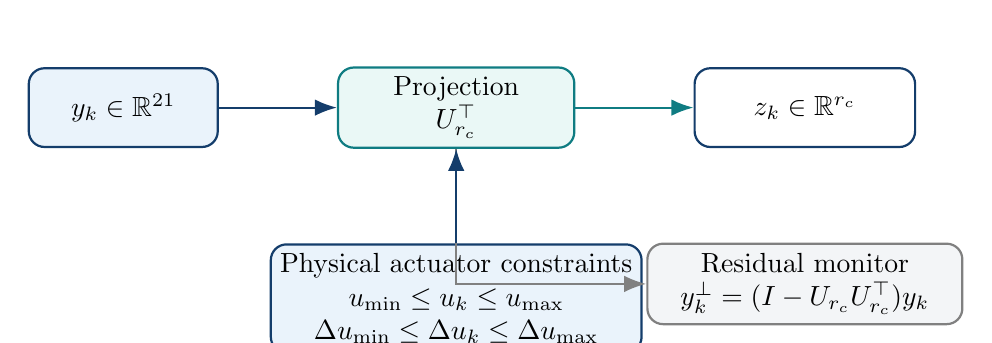
\begin{tikzpicture}[
node distance=9mm and 10mm,
box/.style={draw,rounded corners=2mm,thick,align=center,minimum height=10mm},
arr/.style={-{Latex[length=2.8mm]},thick}
]
\node[box,fill=SoftBlue,draw=TitleBlue,minimum width=24mm] (y) {$y_k\in\R^{21}$};
\node[box,fill=SoftTeal,draw=AccentTeal,right=15mm of y,minimum width=30mm] (proj) {Projection\\$U_{r_c}^\top$};
\node[box,fill=white,draw=TitleBlue,right=15mm of proj,minimum width=28mm] (z) {$z_k\in\R^{r_c}$};
\node[box,fill=SoftGray,draw=gray,below=12mm of z,minimum width=40mm] (res) {Residual monitor\\$y_k^{\perp}=(I-U_{r_c}U_{r_c}^\top)y_k$};
\node[box,fill=SoftBlue,draw=TitleBlue,below=12mm of proj,minimum width=40mm] (u) {Physical actuator constraints\\$u_{\min}\le u_k\le u_{\max}$\\$\Delta u_{\min}\le\Delta u_k\le\Delta u_{\max}$};
\draw[arr,TitleBlue] (y) -- (proj);
\draw[arr,AccentTeal] (proj) -- (z);
\draw[arr,gray] (proj) |- (res.west);
\draw[arr,TitleBlue] (u.north) -- (proj.south);
\end{tikzpicture}
\caption{Modal decomposition is used for performance shaping, but feasibility must remain in the physical actuator coordinates.}
\end{figure}

\section{State-Space Models for Hierarchical Robust Design}
For delayed R2R control, define the augmented supervisory state
\[
x_k=\begin{bmatrix}x_k^{(p)}\\x_k^{(I)}\\x_k^{(d)}\end{bmatrix},
\]
where $x_k^{(p)}$ is the plant or drift state, $x_k^{(I)}$ is the integral tracking state, and $x_k^{(d)}$ is the delay state. A generic realization is
\[
x_{k+1}=Ax_k+B_u u_k+B_w w_k,\qquad y_k=C_yx_k+D_{yu}u_k+D_{yw}w_k.
\]
For offset rejection,
\[
x_{k+1}^{(I)}=x_k^{(I)}+E_I(r_k-y_k).
\]
Mode-selective integral action is preferred over naive full-state integration.

For the faster InRun layer, an analogous realization is
\[
x^{\mathrm{in}}_{k,j+1}=A^{\mathrm{in}}_{k,j}x^{\mathrm{in}}_{k,j}+B^{\mathrm{in}}_{k,j}u_{k,j}+B^{\mathrm{in}}_{w,k,j}w^{\mathrm{in}}_{k,j},
\]
\[
y^m_{k,j}=C^{\mathrm{in}}_{k,j}x^{\mathrm{in}}_{k,j}+D^{\mathrm{in}}_{yw,k,j}w^{\mathrm{in}}_{k,j}.
\]
In deployment, the R2R state initializes each wafer and the InRun state closes the fast loop during that wafer.

\section{Exogenous Inputs and Noise Model}
For the supervisory layer,
\[
w_k=\begin{bmatrix}r_k\\d_k\\n_k\\\eta_k\end{bmatrix},\qquad y_k^m=y_k+n_k,
\]
where $r_k$ is the reference profile, $d_k$ is process disturbance or incoming-wafer variation, $n_k$ is metrology noise, and $\eta_k$ drives uncertainty or scheduling mismatch.
For the InRun layer,
\[
w^{\mathrm{in}}_{k,j}=\begin{bmatrix}r_{k,j}\\d_{k,j}\\n_{k,j}\\\eta_{k,j}\end{bmatrix},\qquad y^m_{k,j}=y_{k,j}+n_{k,j}.
\]

\section{Non-Square MIMO Sensitivity Definitions}
Because $G\in\R^{21\times 11}$, the products $GK$ and $KG$ live in different spaces. Output-side sensitivity and complementary sensitivity are defined by
\[
S_o=(I_{21}+GK)^{-1},\qquad T_o=GK(I_{21}+GK)^{-1}.
\]
Input-side sensitivity and complementary sensitivity are defined by
\[
S_i=(I_{11}+KG)^{-1},\qquad T_i=KG(I_{11}+KG)^{-1}.
\]
In CMP, both profile-quality performance and actuator smoothness matter, so both sides should be reviewed.

\section{Hard Constraints and Anti-Windup}
Physical pressure commands must satisfy
\[
u_{\min}\le u_k\le u_{\max},\qquad u_{\min}\ge 0,
\]
componentwise, and pressure slew must satisfy
\[
\Delta u_{\min}\le u_k-u_{k-1}\le\Delta u_{\max}.
\]
Therefore any unconstrained closed-form expression such as $u_k^{\star}=H_k^{-1}b_k$ can only be interpreted as a pre-saturation candidate, not the final deployable recipe.

When integral action is present and actuator saturation occurs, anti-windup logic is mandatory. With back-calculation,
\[
x_{k+1}^{(I)}=x_k^{(I)}+E_I e_k+K_{aw}(u_k^{\mathrm{sat}}-u_k^{\mathrm{cmd}}),
\]
where $K_{aw}$ is the anti-windup gain matrix. A simpler alternative is conditional integration, in which the integral update is frozen or slowed whenever the integration direction would deepen saturation.

\section{Observer and Estimation Structure}
A generic estimator is
\[
\hat x_{k+1}=A\hat x_k+B_u u_k+L(y_k^m-\hat y_k^m),\qquad \hat y_k^m=C_y\hat x_k+D_{yu}u_k,
\]
where $L$ is the observer gain. Possible strategies include a Kalman filter, an $H_{\infty}$ filter, a reduced-order wear-state estimator, or a hybrid estimator using both metrology and side-channel signals.

When metrology arrives with a delay of $\delta_u$ runs and the measurement received at control step $k$ corresponds to run $k-\delta_u$, define the innovation as
\[
\epsilon_k=y_k^m-\hat y^{m}_{k-\delta_u\mid k-\delta_u-1}.
\]
The delayed estimate is corrected first and then propagated forward to the current run using stored input history. Comparing delayed metrology directly against the current prediction is generally biased and may destabilize adaptation.

\section{Static Constrained Baseline Formulation}
Before dynamic $H_{\infty}$ synthesis, the preferred first deployment baseline is the full-space constrained quadratic program
\begin{align*}
\min_{u_k}\quad &(r_k-G_0u_k)^\top W_e^\top W_e(r_k-G_0u_k)+u_k^\top W_u^\top W_u u_k\\
&\qquad +(u_k-u_{k-1})^\top W_{\Delta u}^\top W_{\Delta u}(u_k-u_{k-1})
\end{align*}
subject to
\[
u_{\min}\le u_k\le u_{\max},\qquad \Delta u_{\min}\le u_k-u_{k-1}\le \Delta u_{\max}.
\]
If reduced-space performance shaping is desired, it should be layered on top of this physical-space baseline rather than replacing it.

\section{Weighting Strategy}
A typical diagonal choice is
\[
W_e=\diag(w_{e,1},\dots,w_{e,21}),\quad W_u=\diag(w_{u,1},\dots,w_{u,11}),\quad W_{\Delta u}=\diag(w_{\Delta u,1},\dots,w_{\Delta u,11}).
\]
Edge-related modes may be weighted more heavily in $W_e$, while retaining-ring or fragile outer-zone action may receive higher penalty in $W_u$. For robust synthesis, one useful multiplicative-uncertainty form is
\[
G_k=G_s(I+W_m\Delta_k),\qquad \norm{\Delta_k}_{\infty}\le 1.
\]

\section{Generalized Plant Construction and $H_{\infty}$ Policy}
The generalized plant is defined by
\[
\begin{bmatrix}z_k\\y_k^m\end{bmatrix}=\begin{bmatrix}P_{11}(z) & P_{12}(z)\\P_{21}(z)&P_{22}(z)\end{bmatrix}\begin{bmatrix}w_k\\u_k\end{bmatrix},
\qquad u_k=K(z)y_k^m,
\]
with the closed-loop interconnection represented by the lower LFT $F_{\ell}(P,K)$. A common performance output is
\[
z_k=\begin{bmatrix}W_e e_k\\W_u u_k\\W_{\Delta u}(u_k-u_{k-1})\\W_n y_k^m\end{bmatrix}.
\]
The explicit partition used by synthesis toolchains is
\begin{align*}
x_{k+1} &= A_Px_k+B_{P1}w_k+B_{P2}u_k,\\
z_k &= C_{P1}x_k+D_{P11}w_k+D_{P12}u_k,\\
y_k^m &= C_{P2}x_k+D_{P21}w_k+D_{P22}u_k.
\end{align*}
Because the baseline loop is indexed by run number, the preferred synthesis framework is discrete-time $H_{\infty}$ design with target
\[
\norm{T_{zw}(z)}_{\infty}<\gamma,
\]
interpreted on the unit circle $z=\e^{j\omega}$.

\begin{figure}[h!]
\centering
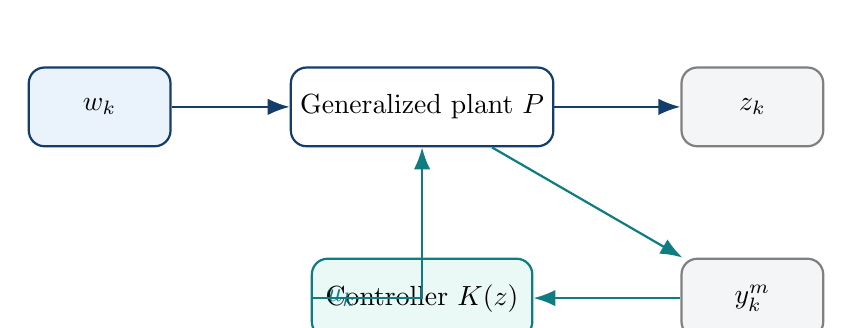
\begin{tikzpicture}[
node distance=8mm and 10mm,
box/.style={draw,rounded corners=2mm,thick,align=center,minimum height=10mm},
arr/.style={-{Latex[length=2.8mm]},thick}
]
\node[box,fill=SoftBlue,draw=TitleBlue,minimum width=18mm] (w) {$w_k$};
\node[box,fill=white,draw=TitleBlue,right=15mm of w,minimum width=32mm] (P) {Generalized plant $P$};
\node[box,fill=SoftTeal,draw=AccentTeal,below=14mm of P,minimum width=28mm] (K) {Controller $K(z)$};
\node[box,fill=SoftGray,draw=gray,right=16mm of P,minimum width=18mm] (z) {$z_k$};
\node[box,fill=SoftGray,draw=gray,below=14mm of z,minimum width=18mm] (y) {$y_k^m$};
\draw[arr,TitleBlue] (w) -- (P);
\draw[arr,TitleBlue] (P) -- (z);
\draw[arr,AccentTeal] (P) -- (y);
\draw[arr,AccentTeal] (y) -- (K);
\draw[arr,AccentTeal] (K.west) -| node[pos=0.25,left,] {$u_k$} (P.south);
\end{tikzpicture}
\caption{Explicit generalized-plant interconnection used for discrete-time $H_{\infty}$ synthesis and implementation.}
\end{figure}

\section{Pseudoinverse and Identification Notes}
Any use of normalized residuals such as $G_iG_0^{\dagger}-I$ must state the pseudoinverse convention explicitly. For initial uncertainty analysis, direct additive residuals are safer:
\[
\Delta G_i=G_i-G_0.
\]
A more numerically disciplined relative-comparison route is to compare reduced plants,
\[
\widetilde G_i=U_{r_c}^\top G_i,
\]
before computing deviations.

\section{Implementation Roadmap}
\begin{enumerate}[leftmargin=1.7em]
\item \textbf{Phase 1 --- InRun sensing and identification}: identify usable in-situ signals, map them to profile estimates, identify turn-wise response matrices $H_{k,j}$ or an equivalent in-run state-space model, and quantify latency.
\item \textbf{Phase 2 --- InRun constrained baseline}: deploy a turn-wise constrained controller with hard pressure and slew limits, verify target tracking against measured turn-by-turn error, and characterize disturbance rejection.
\item \textbf{Phase 3 --- Supervisory R2R adaptation}: identify $G_0$, quantify metrology delay, collect wear covariates, compute the SVD, and update the wafer-level baseline recipe generation.
\item \textbf{Phase 4 --- Integrated robust controller}: connect the InRun and R2R layers through a consistent generalized-plant description, then synthesize reduced-order discrete-time robust controllers and filters.
\item \textbf{Phase 5 --- Scheduled/adaptive predictive control}: schedule the plant with wear state, update the nominal model online, and move toward robust MPC when constraints and preview information dominate.
\end{enumerate}

\begin{figure}[h!]
\centering
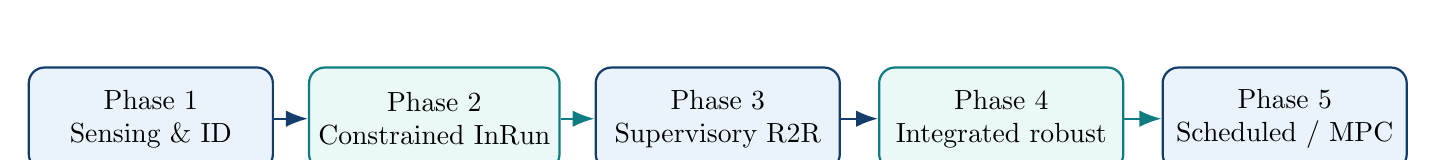
\begin{tikzpicture}[
phase/.style={draw,rounded corners=2mm,thick,minimum width=31mm,minimum height=13mm,align=center},
arr/.style={-{Latex[length=2.8mm]},thick}
]
\node[phase,fill=SoftBlue,draw=TitleBlue] (p1) at (0,0) {Phase 1\\Sensing \& ID};
\node[phase,fill=SoftTeal,draw=AccentTeal] (p2) at (3.6,0) {Phase 2\\Constrained InRun};
\node[phase,fill=SoftBlue,draw=TitleBlue] (p3) at (7.2,0) {Phase 3\\Supervisory R2R};
\node[phase,fill=SoftTeal,draw=AccentTeal] (p4) at (10.8,0) {Phase 4\\Integrated robust};
\node[phase,fill=SoftBlue,draw=TitleBlue] (p5) at (14.4,0) {Phase 5\\Scheduled / MPC};
\draw[arr,TitleBlue] (p1) -- (p2);
\draw[arr,AccentTeal] (p2) -- (p3);
\draw[arr,TitleBlue] (p3) -- (p4);
\draw[arr,AccentTeal] (p4) -- (p5);
\end{tikzpicture}
\caption{Recommended deployment path from constrained baseline to integrated robust and predictive control.}
\end{figure}

\section{Verification Plan}
Verification must cover both wafer-level and turn-level behavior: target-profile tracking within the same wafer, edge suppression, smooth pressure trajectories, and convergence in reduced modal coordinates. Robustness tests should include pad wear drift, retaining-ring wear drift, slurry perturbation, delayed post-metrology, InRun sensing latency, real-time disturbance bursts, and input saturation. Structural tests should explicitly check controllable versus uncontrollable mode separation, observer detectability, anti-windup behavior, coordination between the InRun and R2R layers, and constraint-feasibility statistics. Useful deployment metrics include turn-wise RMS profile error, final-wafer RMS residual, edge residual, null-space residual energy, saturation frequency, pressure-move norm, disturbance-rejection settling time, and recovery after saturation.

\section{Design Conclusions}
This specification adopts the following practical position:
\begin{enumerate}[leftmargin=1.7em]
\item CMP profile control should be treated first as an InRun robust-tracking problem with a slower R2R supervisory layer.
\item The plant is not merely uncertain but also slowly time-varying across wafers and disturbed in real time within the same wafer.
\item Since $G\in\R^{21\times 11}$, design must explicitly account for controllable shape modes and uncontrollable residual modes.
\item The controller must define a target profile, measure turn-wise deviation from that target, and compute bounded pressure corrections at each turn.
\item Any deployable controller must respect hard pressure non-negativity and rate constraints at both the InRun and wafer levels.
\item Integral action is acceptable only with explicit anti-windup protection, and observer design must address both delayed post-metrology and faster in-situ estimates.
\item The generalized plant must be assembled in an explicit discrete-time partitioned state-space form.
\item The recommended practical path is summarized below.
\begin{align*}
&\text{InRun constrained tracking baseline}\\
\rightarrow\;&\text{R2R supervisory adaptation}\\
\rightarrow\;&\text{Integrated reduced-order discrete-time } H_{\infty}\\
\rightarrow\;&\text{Gain-scheduled / adaptive robust control}\\
\rightarrow\;&\text{Robust MPC if constraints dominate.}
\end{align*}
\end{enumerate}

\appendix
\section{Immediate Additions Recommended for Production Review}
The following items remain mandatory for a production-grade review package:
\begin{enumerate}[leftmargin=1.7em]
\item InRun sensing-latency and observability table.
\item Metrology-delay table.
\item Actuator-bound table.
\item Turn-wise target-profile definition note.
\item SVD truncation criterion.
\item Observer-realization note.
\item Anti-windup implementation note.
\item Generalized-plant matrix appendix.
\item Wear-state scheduling policy.
\end{enumerate}

\section{Minimal Deployable Baseline}
If a first deployment must be executed quickly, the minimum defensible path is:
\begin{enumerate}[leftmargin=1.7em]
\item define the InRun target profile or target trajectory,
\item build an observer for turn-wise profile estimation from available in-situ signals,
\item solve a constrained InRun tracking problem with $u_{\min}\ge 0$,
\item add back-calculation anti-windup and turn-wise slew limiting,
\item measure the effective post-metrology delay $\delta_u$,
\item use R2R adaptation as the slower supervisory correction layer.
\end{enumerate}

\end{document}
